\documentclass[12pt,compress,aspectratio=169]{beamer}

\mode<presentation>
{
  \usetheme{Singapore}
%  \setbeamertemplate{navigation symbols}{} % suppress nav bar
%  \setbeamercovered{transparent}
}
\usefonttheme{professionalfonts}
\usepackage{graphicx}
\usepackage{tikz}
\usepackage{amsmath}
\usepackage{mathpazo}
\usepackage[scaled]{helvet}
\usepackage{xcolor,colortbl}
\usepackage{hyperref}
\usepackage{siunitx}

\sisetup{
  number-math-rm=\mathnormal,
  per-mode=symbol
}

\title{Topic 23: Special Relativity}
\subtitle{Advanced Placement Physics}
\author[TML]{Dr.\ Timothy Leung}
\institute{Olympiads School}
%\author{Olympiads School}
\date{Summer 2018}




\newcommand{\mb}[1]{\mathbf{#1}}
\newcommand{\pic}[2]{\includegraphics[width=#1\textwidth]{#2}}
\newcommand{\bigsqrt}{\ensuremath\sqrt{1-\left(\frac{v}{c}\right)^2}}
\newcommand{\lorentz}{\ensuremath\frac{1}{\bigsqrt}}
\newcommand{\eq}[2]{\vspace{#1}{\Large\begin{displaymath}#2\end{displaymath}}}



\begin{document}

\begin{frame}
  \maketitle
\end{frame}



\section[Intro]{Introduction}
\begin{frame}
  \frametitle{Introduction}
  The slides on \textbf{special relativity} is an expanded version of the
  slides used for Physics 12 (and with some calculus). For many of you, this is
  a review. There are 2 versions of the slides that are downloadable from
  the school website:
  \begin{itemize}
  \item The long version
    \begin{itemize}
    \item More background information and derivations and integrations
    \item \texttt{23a-relativity\_long.pdf}
    \end{itemize}
  \item The short version
    \begin{itemize}
    \item More ``to the point''
    \item The version that I am using in this class
    \item \texttt{23a-relativity\_short.pdf}
    \end{itemize}
  \end{itemize}
  There is also a handout on how to solve and interpret the time dilation
  example problem.
\end{frame}


\begin{frame}
  \frametitle{Frame of Reference}
  A \textbf{frame of reference} is a hypothetical mobile ``laboratory'' an
  observer uses to make measurements (e.g.\ mass, lengths, time). At a minimum,
  it must include:
  \begin{itemize}
  \item A ruler to measure lengths
  \item A clock to measure the passage of time
  \item A scale to compare forces
  \item A balance to measure masses
  \end{itemize}
  \textcolor{red!85}{High-school textbooks often refer to the frame of reference
    as a ``coordinate system''. While it certainly includes that, this
    definition often makes it difficult to understand special relativity.}
\end{frame}


\begin{frame}
  \frametitle{Frame of Reference}
  \begin{itemize}
  \item We assume that the hypothetical laboratory is \emph{perfect}
  \item What ``instruments'' are used are unimportant
  \item What matters is the \emph{motion} (at rest, uniform motion, acceleration
    etc) of your laboratory, and how it affects the measurement that you make
  \item ``From the point of view of\ldots''
  \end{itemize}
\end{frame}


\begin{frame}
  \frametitle{Frame of Reference}
  Although both observers see different motion, but they agree on the equations
  that goven the motion (laws of motion).
  \begin{center}
    \pic{.75}{graphics/57.jpg}
  \end{center}
\end{frame}

\begin{frame}
  \frametitle{Newtonian (Classical) Relativity}

  In Newtonian physics, space and time are \emph{absolute}:
  \begin{itemize}
  \item \SI{1}{m} is \SI{1}{m} no matter where you are in the universe
  \item \SI{1}{s} is \SI{1}{s} no matter where you are in the universe
  \item Measurements of space and time do not depend on motion
  \end{itemize}
  If space and time are absolute, then \emph{all} velocities are relative
  \begin{itemize}
  \item Measured velocities depend on the motion of the observer
  \item An \textbf{inertial} frame of reference moving in uniform motion
    (constant velocity,  without acceleration)
  \end{itemize}

  \vspace{.2in}
  \begin{block}{The Principle of Relativity}
    All laws of physics must apply equally in all inertial frames of reference.
  \end{block}
\end{frame}

\begin{frame}
  \frametitle{New Physics: Maxwell's Equations}
  \begin{columns}
    \column{0.3\textwidth}
    \begin{center}
      \pic{1}{graphics/PORTRAIT-James-Clerk-Maxwell.jpg}\\
      James Clerk Maxwell
    \end{center}
    \column{0.7\textwidth}
    \begin{itemize}
    \item Classical laws of electrodynamics
    \item Published in 1861 and 1862
    \item Explains the relationship between
      \begin{itemize}
      \item Electricity
      \item Electric Circuits
      \item Magnetism
      \item Optics
      \end{itemize}
    \item Previously these disciplines are thought to be separate and not
      related
    \end{itemize}
  \end{columns}
\end{frame}


\begin{frame}
  \frametitle{Maxwell's Equations in a Vacuum}
  \framesubtitle{Everything Comes Back to This}

  \vspace{-.3in}{\Large
    \begin{align*}
      \nabla\cdot\mb{E} &= 0\\
      \nabla\cdot\mb{B} &= 0\\
      \nabla\times\mb{E} &=-\frac{\partial\mb{B}}{\partial t}\\
      \nabla\times\mb{B} &=\mu_0\varepsilon_0\frac{\partial\mb{E}}{\partial t}
    \end{align*}
  }
  
  \vspace{-.15in}Disturbances in $\mb{E}$ and $\mb{B}$ travel as an
  ``electromagnetic wave'', with a speed:

  \vspace{-.25in}{\Large
    \begin{displaymath}
      c=\frac{1}{\sqrt{\varepsilon_0\mu_0}}=\SI{299792458}{m/s}
    \end{displaymath}
  }
\end{frame}


\begin{frame}
  \frametitle{Peculiar features of Maxwell's equation}
  \begin{itemize}
  \item Makes no mention of the \emph{medium} in which EM waves travels
  \item When applying \emph{Galilean transformation} (classical equation for
    calculating \emph{relative velocity}) to Maxwell's equations, asymmetry is
    introduced
  \item Gauss's law for magnetism break down: magnetic field lines appear to
    have beginnings/ends
  \item In \emph{some} inertial frames of reference,
    Maxwell's equations are simple and elegant, but in another inertial frame
    of reference, they are ugly and complex
  \item Physicists at the time theorized that---perhaps---there is/are actually
    \emph{preferred} inertial frame(s) of references
  \item This violate the \emph{principle of relativity}
  \end{itemize}
\end{frame}


\begin{frame}
  \frametitle{The Illusive Aether}
  \begin{itemize}
  \item Maxwell's hypothesis: the speed of light $c_0$ is relative to a
    hypothetical ``luminiferous aether''
  \item In order for this ``aether'' (or ``ether'') to exist, it must have some
    fantastic (as in, a fantasy, too good to be true!) properties:
    \begin{itemize}
    \item \emph{All} space is filled with aether
    \item Massless
    \item Zero viscosity
    \item Non-dispersive
    \item Incompressible
    \item Continuous at a very small (sub-atomic) scale
    \end{itemize}
  \end{itemize}
\end{frame}



\begin{frame}
  \frametitle{The Michelson-Morley Experiment}
  If ether exists, then at different times of the year, the Earth will have a
  different relative velocity with respect to it:
  \begin{center}
    \pic{.45}{graphics/2000px-AetherWind.png}
  \end{center}
  And it will cause light to either speed up, or slow down.
\end{frame}



\begin{frame}
  \frametitle{The Michelson Interferometer}
  \pic{1}{graphics/michelsonmorley.jpg}\\
  The experiment is ingenious but very difficult\ldots
\end{frame}



\begin{frame}
  \frametitle{The Michelson Interferometer}
  \begin{columns}
    \column{.35\textwidth}
    \begin{center}
      \pic{1.1}{graphics/313754.jpg}
    \end{center}

    \column{.65\textwidth}
    \begin{itemize}
    \item A beam of light is split into two using a two-way (half-silvered)
      mirror
    \item The two beams are reflected off mirrors and finally arriving at the
      screen where interference patterns are observed
    \item The two paths are the same length, so if the \emph{speed} of the light
      changes, we should see an interference pattern
    \item\textbf{Except none were ever found!}
    \end{itemize}
  \end{columns}
\end{frame}



\begin{frame}
  \frametitle{What To Do with ``Null Result''}
  The Michelson-Morley experiment failed to detect the illusive ether, even
  after many refinements. What does this mean?
  \begin{itemize}
  \item Majority view
    \begin{itemize}
    \item\textbf{The experiment was flawed!}
    \item Keep improving the experiment (or design a better experiment) and the
      ether will eventually be found
    \end{itemize}
  \item Minority view:
    \begin{itemize}
    \item\textbf{The hypothesis is wrong!}
    \item The experiment showed it for what it is: ether cannot be found
    \end{itemize}
  \item A few physicists: The must be \textbf{another explanation} that saves
    both experiment and theory
  \end{itemize}
\end{frame}



\begin{frame}
  \frametitle{Hendrik Lorentz}
  \begin{columns}
    
    \column{0.25\textwidth}
    \begin{center}
      \pic{1.2}{graphics/lorentz.jpg}\\
      {\footnotesize Hendrik Antoon Lorentz}
    \end{center}
    
    \column{0.75\textwidth}
    \begin{itemize}
    \item Considered the Michelson-Morley experiment to be significant
    \item Objects travelling in the direction of ether contracts in length,
      nullifying the experimental results
    \item Lorentz Factor:
      
      \eq{-.25in}{
        \boxed{\gamma=\lorentz}
      }
    \item \emph{No known physical phenomenon} can cause anything to contract
    \item Lorentz was on to something, but his thinking was wrong
    \end{itemize}
  \end{columns}
\end{frame}

\begin{frame}
  \frametitle{Making Maxwell's Equations Work}
  \framesubtitle{Albert Einstein in 1905, Age 26}
  \begin{columns}
    \column{.25\textwidth}
    \pic{1.1}{graphics/Einstein_patentoffice.jpg}\\
    {\footnotesize Albert Einstein}
  
    \column{0.75\textwidth}
    \begin{itemize}
    \item Einstein believed in the principle of relativity, and therefore
      rejected the concept of a preferred frame of reference
    \item The failure of the Michelson-Morley experiment to find the flow of
      ether proves that it does not exist
    \item In order to make the equations to work again, Einstein revisited two
      most fundamental concepts in physics: space and time
    \end{itemize}
  \end{columns}
\end{frame}



\begin{frame}
  \frametitle{Special Relativity}
  \begin{itemize}
  \item Largely ignored by most physicists at first, until Max Planck took an
    interest in it
  \item Soon adopted by many physicists
  \item ``Special'' relativity because it describes a ``special case'' without
    effects of forces (e.g.\ gravity) \& acceleration
  \item Later published theory of ``general relativity'' (much more complicated)
  \end{itemize}
\end{frame}



\begin{frame}
  \frametitle{Postulates}
  \begin{block}{The Principle of Relativity}
    All laws of physics must apply equally in all inertial frames of reference.
  \end{block}

  \begin{block}{The Principle of Invariant Light Speed}
    As measured in any inertial frame of reference, light is always propagated
    in empty space with a definite velocity $c$ that is independent of the
    state of motion of the emitting body.
  \end{block}

  \vspace{.15in}Published in the journal \emph{Annalen der Physik} on September
  26, 1905 in the article \emph{On the Electrodynamics of Moving Bodies} when
  Einstein was 26 years old working as a patent clerk in Switzerland
\end{frame}

\begin{frame}
  \frametitle{What's so Special About Special Relativity?}

  \textbf{Classical (Newtonian) relativity:}
  \begin{itemize}
  \item Space and time are absolute, therefore
  \item The speed of light must be relative to the observer
  \end{itemize}

  \textbf{Einstein's special relativity:}
  \begin{itemize}
  \item The speed of light is absolute, therefore
  \item Space and time must be relative to the observer
  \end{itemize}

  We must modify our traditional concepts:
  \begin{itemize}
  \item Measurement of space (our ruler in the $x$-, $y$- and $z$-directions)
  \item Measurement of time (our clock)
  \item Concept of simultaneity (whether two events happens at the same time)
  \end{itemize}
\end{frame}

%\begin{frame}
%  \frametitle{Simultaneity: Thought Experiment}
%  If you see two sets of fire works ignite at exactly the same time--one off to
%  your left and the other far to your right. About \SI{100}{\metre} behind you,
%  a car is travelling along a highway at \SI{95}{km/h}. Do the passengers in
%  the car see the fire works igniting simultaneously or do they think that one
%  set ignited before the other?
%\end{frame}

\section{Simultaneity}

\begin{frame}
  \frametitle{Simultaneity: Thought Experiment}
  Lightning bolt strikes the ends of a moving train
  \begin{center}
    \pic{.5}{graphics/87-1-1024x673.png}
  \end{center}
  \vspace{-0.1in}
  \begin{itemize}
  \item The man on the ground sees the lightning bolt striking at the same time
  \item The woman on the moving train sees the lightning bolt on the right first
  \end{itemize}
\end{frame}

% PUT IN NEW SLIDES ON SIMULTANEITY HERE!


\begin{frame}
  \frametitle{Simultaneity: Thought Experiment}
  \begin{itemize}
  \item The two observers disagree on the result, but
    \begin{itemize}
    \item Neither person is wrong
    \item Neither person is misinformed
    \end{itemize}
  \item Both observers are valid \emph{inertial} frames of reference
  \item This means that simultaneity depends on your motion
  \end{itemize}
  
  \vspace{.2in}\textbf{Events that are simultaneous in one inertial frame of
    reference are not simultaneous in another.}
\end{frame}



\section{Time Dilation}

\begin{frame}
  \frametitle{Time Dilation: A Thought Experiment}
  \begin{center}
    \pic{.7}{graphics/spaceship.png}
    %\pic{.4}{graphics/light-a-b.png}
  \end{center}
  I'm on a spaceship travelling in deep space, and I shine a light from
  $A$ to $B$. The distance between $A$ and $B$ is really just:

  \vspace{-.3in}{\Large
    \begin{displaymath}
      |AB|=ct
    \end{displaymath}
  }

  \vspace{-.2in}I know the speed of light $c$, and I know how long it took for
  the light pulse to reach $B$.
\end{frame}


\begin{frame}
  \frametitle{Time Dilation: A Thought Experiment}
  \begin{center}
    \pic{.7}{graphics/spaceship.png}
    %\pic{.7}{graphics/light-a-b-rocket.png}
  \end{center}
  You are in space station watching my spaceship go past you at speed $v$. You
  would see that same beam of light travel from $A$ to $B'$ instead.
  \begin{center}
    \pic{.7}{graphics/light-a-b-prime.png}
  \end{center}
\end{frame}

\begin{frame}
  \frametitle{Time Dilation: A Thought Experiment}
  \begin{center}
    \pic{.7}{graphics/dilation.png}
  \end{center}
  \begin{align*}
    c^2\Delta t^2 &=v^2\Delta t^2 + c^2\Delta t_0^2\\
    \left(c^2-v^2\right)\Delta t^2 &=c^2\Delta t_0^2\\
    \left(1-\frac{v^2}{c^2}\right)\Delta t^2 &=\Delta t_0^2\\
    \Delta t &=\frac{\Delta t_0}{\bigsqrt}
  \end{align*}
\end{frame}


\begin{frame}
  \frametitle{Time Dilation: A Thought Experiment}
  
  \eq{-.2in}{
    \boxed{t' =\frac{t}{\bigsqrt}}
  }
  \begin{itemize}
  \item $t$ is called the \textbf{proper time}. It is the time measured
    by a person at rest relative to the object or event.
  \item $t'$ is called the expanded time or \textbf{dilated time}. It is 
    the time measured by a moving observer in another inertial frame of
    reference. Since $\bigsqrt$ is always smaller than 1, $t'$ is always
    greater than $t$.
  \end{itemize}
\end{frame}

\begin{frame}
  \frametitle{Example Problem}
  \textbf{Example 1a:} A rocket speeds past an asteroid at $0.800c$. If an
  observer in the rocket sees \SI{10.0}{s} pass on her watch, how long would
  that time interval be as seen by an observer on the asteroid?


  \uncover<2->{
    \vspace{.3in}\textbf{Example 1b:} A rocket speeds past an asteroid at
    $0.800c$. If an observer in the \emph{asteroid} sees \SI{10.0}{s} pass on
    his watch, how long would that time interval be as seen by an observer on
    the \emph{rocket}?
  }

  \uncover<3->{
    \vspace{.3in}How can that be?!
  }
\end{frame}


\section{Length Contraction}

\begin{frame}
  \frametitle{Abandoning Concept of Absolute Space: Length Contraction}
  \framesubtitle{Another Example}
  Captain Quick is a comic book hero who can run at nearly the speed of light.
  In his hand, he is carrying a flare with a lit fuse set to explode in
  \SI{1.5}{\micro\second}. The flare must be placed into its bracket before this
  happens. The distance ($L$) between the flare and the bracket is
  \SI{402}{\metre}.
\end{frame}

\begin{frame}
  \frametitle{Abandoning Concept of Absolute Space: Length Contraction}
  \framesubtitle{Another Example}
  \begin{center}
    \pic{0.85}{graphics/captain-quick.png}
  \end{center}
\end{frame}


\begin{frame}
  \frametitle{Abandoning Concept of Absolute Space: Length Contraction}
  \framesubtitle{Another Example}
  If Captain Quick runs at \SI{2.00e8}{m/s}, according to classical mechanics,
  he will not make it in time:
  \begin{displaymath}
    t= \frac{L}{v}=\frac{\SI{402}{m}}{\SI{2.00e8}{m/s}}
    =\SI{2.01e-6}{s}=\SI{2.01}{\micro s}
  \end{displaymath}
  But according to relativistic mechanics, he makes it just in time\ldots
\end{frame}

\begin{frame}
  \frametitle{Abandoning Concept of Absolute Space: Length Contraction}
  \framesubtitle{Another Example}
  To a stationary observer, the time on the flare is slowed:
  \begin{displaymath}
    t'
    = \frac{t}{\bigsqrt}
    = \frac{\SI{1.5e-6}{s}}{\sqrt{1-\left(\frac{2}{3}\right)^2}}
    = \frac{\SI{1.5e-6}{s}}{0.7454}
    = \SI{2.01e-6}{s}
  \end{displaymath}
  The stationary observer sees a passage of time of
  $t'=\SI{2.01}{\micro\second}$, but
  Captain Quick, who is in the same reference frame as the flare, experiences
  a passage of time of $t=\SI{1.50}{\micro\second}$, precisely the
  time for the flare to explode.
\end{frame}

\begin{frame}
  \frametitle{Abandoning Concept of Absolute Space: Length Contraction}
  \framesubtitle{Another Example}
  \begin{itemize}
  \item So, if Captain Quick sees only $t=\SI{1.50}{\micro s}$, then
    how far did he travel?
  \item He isn't travelling any faster, so he only other possibility is that
    \textbf{the distance actually got shorter} (in his frame of reference).
  \item How much did the distance contract?
  \end{itemize}
  
  \eq{-.2in}{
    \boxed{L'=L\bigsqrt}
  }

  For this example:
  \begin{displaymath}
    L'=L\bigsqrt=(\SI{402}{m})\cdot\sqrt{1-\left(\frac{2}{3}\right)^2}
    =\SI{300}{m}
  \end{displaymath}
\end{frame}


\section{Lorentz Factor}

\begin{frame}
  \frametitle{Lorentz Factor}
  The \textbf{Lorentz factor} $\gamma$ is a short-hand for writing length
  contraction, time dilation and relativistic mass:

  \eq{-.2in}{
    \boxed{\gamma=\lorentz}
  }
  
  Then time dilation and length contraction can be written simply as:
  
  \eq{-.1in}{
    \boxed{t' = \gamma t}\quad\boxed{L' = \frac{L}{\gamma}}
  }
\end{frame}

\begin{frame}
  \frametitle{Let's Summarize}
  \begin{center}
    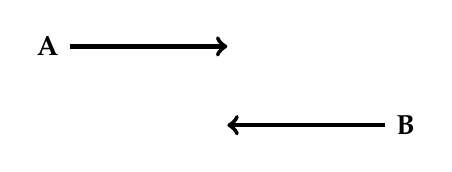
\begin{tikzpicture}[scale=2]
      \draw[ultra thick,->] (1,.5)--(2,.5) node[pos=0,left] {\textbf{A}};
      \draw[ultra thick,->] (3,0)--(2,0) node[pos=0,right]{\textbf{B}};
    \end{tikzpicture}
  \end{center}
  If Person A and Person B are moving at constant speed with respect to one 
  another (doesn't matter if they're moving towards, or away from each other)
  \begin{itemize}
  \item They cannot agree whether any events happens at the same time or not
  \item Each sees the other's clock running slow
  \item Each sees the other ``contracted'' in length along the direction of
    motion
  \end{itemize}
\end{frame}

\begin{frame}
  \frametitle{Example Problem}
  \textbf{Example 2:} A spacecraft passes Earth at a speed of \SI{2.00e8}{m/s}.
  If observers on Earth measure the length of the spacecraft to be
  \SI{554}{m}, how long would it be according to its passengers?
\end{frame}



\section[Momentum]{Relativistic Momentum}

\begin{frame}
  \frametitle{Relativistic Momentum}
  In Physics 12, you were taught that momentum is mass times velocity. And back
  in Physics 11, you were taught that velocity is displacement over time.
  \textbf{These definitions have not changed.}

  \eq{-.2in}{
    \mb{p}=m\frac{d\mb{x}}{dt}
  }

  \vspace{-.1in}But now that you know $d\mb{x}$ and $dt$ depend on motion, we
  can find the ``relativistic momentum'':
  
  \eq{-.2in}{
    \mb{p}=m\frac{d\mb{x}}{dt}
    =\frac{md\mb{x}}{\bigsqrt\;dt}
    =\frac{m\mb{v}}{\bigsqrt}
  }
\end{frame}


\section[Mass]{Relativistic Mass}

\begin{frame}
  \frametitle{Relativistic Mass}
  From the relativistic momentum expression, we can see that there is a
  relativistic aspect to mass as well. The apparent mass $m'$ as measured by a
  moving observer is related to its rest mass by the Lorentz factor:

  \eq{-.18in}{
    \boxed{m'=\frac{m}{\bigsqrt}=\gamma m}
  }
  
  The real (intrinsic) mass has not increased, but a moving observer will note
  that the object behaves as if it is more massive. As $v\rightarrow c$,
  $m\rightarrow\infty$!
\end{frame}



\section[Energy]{Relativistic Energy}

\begin{frame}
  \frametitle{Force and Work}
  In Physics 12, you were taught that force is the rate of change of momentum
  with respect to time. \textbf{This definition has not changed.}

  \eq{-.2in}{
    \mb{F}=\frac{d\mb{p}}{dt}
  }

  \vspace{-.1in}and that work is the integral of the dot product between force
  and displacement vectors:

  \eq{-.3in}{
    W=\int\mb{F}\cdot d\mb{x}=\int\frac{d\mb{p}}{dt}\cdot \mb{dx}
  }

  \vspace{-.1in}Since we now have a relativistic expression for momentum, we
  substitute that new expression into the expression for force, and then
  integrate.
\end{frame}


\begin{frame}
  \frametitle{Work and Energy}
  For 1D motion, we can rearrange the terms in the integral:

  \eq{-.2in}{
    W=\int Fdx=\int\frac{dp}{dt}dx=\int vdp
  }
  
  \vspace{-.15in}Assuming that both velocity and momentum are continuous in
  time. Since momentum is a function of both $\gamma$ and $v$, we must apply the
  chain rule to find the infinitesimal change in momentum ($dp$) with respect
  to $d\gamma$ and $dv$:
  
  \eq{-.25in}{
    p=\gamma mv \quad\rightarrow\quad dp= \gamma dv +vd\gamma
  }

  \vspace{-.15in}Substitiuting that into the integral, we have:
  
  \eq{-.25in}{
    W=\int vdp=\int mv(\gamma dv +vd\gamma)=
    \int m\left(\gamma vdv +v^2d\gamma\right)
  }
\end{frame}

\begin{frame}
  \frametitle{Work and Energy}
  %The $d\gamma$ term requires some careful (but not very difficult) derivation:
  %
  %\eq{-.3in}{
  %  \gamma=\lorentz\quad\rightarrow\quad
  %  d\gamma=\frac{v/c^2}{(1-v^2/c^2)^{3/2}}dv
  %}

  We want to integrate with respect to $\gamma$, so we need to express $v$
  and $dv$ in terms of $\gamma$ using its definition:

  \eq{-.2in}{
    v^2=c^2\left[1-\left(\frac{1}{\gamma}\right)^2\right]
    \quad\quad
    dv=\frac{c^2}{\gamma^3v}d\gamma
  }
\end{frame}

\begin{frame}
  \frametitle{Work and Energy}
  Putting everything together, we have

  \eq{-.25in}{
    W=\int m(\gamma vdv +v^2d\gamma)=\int m\left[\frac{c^2}{\gamma^2}+
      c^2\left(1-\frac{1}{\gamma^2}\right)\right]d\gamma
  }

  We end up with a surprisingly simple integral:

  \eq{-.2in}{
    W=\int_1^\gamma mc^2d\gamma
  }

  The limit of the integral is from $1$ because at $v=0$, $\gamma=1$
\end{frame}

\begin{frame}
  \frametitle{Work and Kinetic Energy}

  The integral gives us this expression:
  
  \eq{-.15in}{
    W=\gamma mc^2-mc^2 = K
%    W=\frac{mc^2}{\bigsqrt}-mc^2 = K
  }

  \vspace{-.15in}We know from the work-kinetic energy theorem that the work $W$
  done is equal to the change in kinetic energy $K$, therefore
  
  \eq{-.2in}{ \boxed{K=m'c^2-mc^2} }

  \vspace{-.1in}
  \begin{center}
    \begin{tabular}{l|c|c}
      \rowcolor{pink}
      \textbf{Variable} & \textbf{Symbol} & \textbf{SI Unit}\\ \hline
      Kinetic energy of an object & $K$  & \si{\joule}\\
      Relativistic mass (measured in moving frame) & $m'$ & \si{\kilo\gram}\\
      Rest mass (measured in stationary frame) & $m$  & \si{\kilo\gram}\\
      Speed of light              & $c_0$ & \si{\metre\per\second}
    \end{tabular}
  \end{center}
\end{frame}

\begin{frame}
  \frametitle{Relativistic Energy}
  \framesubtitle{What This All Means}
  {\Large
    \begin{displaymath}
      \boxed{K=m'c^2-mc^2}
    \end{displaymath}
  }

  The minimal energy that any object has, regardless of it's motion (or lack
  of) is its \textbf{rest energy}:
  
  \eq{-.4in}{ E_0=mc^2 }

  \vspace{-.2in}The \textbf{total energy} of an object has is
    
  \eq{-.3in}{
    E_T=m'c^2=\gamma mc^2
  }

  \vspace{-.2in}The difference between total energy and rest energy is the
  kinetic energy:

  \eq{-.3in}{
    K=E_T-E_0
  }
\end{frame}


\begin{frame}
  \frametitle{Relativistic Energy}
  \framesubtitle{What This All Means}
  
  \eq{-.2in}{
    \boxed{E=mc^2}
  }

  \textbf{Mass-energy equivalence}:
  \begin{itemize}
  \item Whenever there is a change of energy, there is also a change of mass
  \item ``Conservation of mass'' and ``conservation of energy'' must be
    combined into a single concept of \textbf{conservation of mass-energy}
  \item Mass-energy equivalence doesn't merely mean that mass can be converted
    into energy, and vice versa (although this is true), but rather, one can be
    converted into the other
    \textbf{because they are fundamentally the same thing}
  \end{itemize}
\end{frame}



\begin{frame}
  \frametitle{Example Problem}
  \textbf{Example 3:} An electron has a rest mass of \SI{9.11e-31}{\kilo\gram}.
  In a detector, it behaves as if it has a mass of \SI{12.55e-31}{\kilo\gram}.
  How fast is that electron moving relative to the detector?
\end{frame}


\begin{frame}
  \frametitle{Kinetic Energy--Classical vs.\ Relativistic}
  \begin{columns}
    \column{.5\textwidth}
    \textbf{Relativistic:}
    {\Large
      \begin{displaymath}
        K=\frac{mc^2}{\bigsqrt}-mc^2
      \end{displaymath}
    }
    
    \column{.5\textwidth}
    \textbf{Newtonian:}
    {\Large
      \begin{displaymath}
        K=\frac{1}{2}mv^2
      \end{displaymath}
    }
  \end{columns}
  But are they really that different?
  \begin{itemize}
  \item If space and time are indeed relative quantities, then the relativistic
    equation for $K$ must apply to all velocities
  \item But we know that when $v\ll c$, the Newtonian expression works perfectly
  \item i.e.\ The Newtonian expression for $K$ must be a very good approximation
    for the relativistic expression for $K$ for $v\ll c$
  \end{itemize}
\end{frame}


\begin{frame}
  \frametitle{Binomial Series Expansion}
  The \textbf{binomial series} is the Maclaurin series for the function
  $f(x)=(1+x)^\alpha$, given by:
  
  \eq{-.3in}{
    (1+x)^\alpha=\sum_{k=0}^\infty\left(
    \begin{matrix}
      \alpha\\
      k
    \end{matrix}
    \right)
    x^k=1+\alpha x + \frac{\alpha(\alpha-1)}{2!}x^2+\cdots
  }

  \vspace{-.15in}In the case of relativistic kinetic energy, we use:

  \eq{-.2in}{
    x=-\left(\frac{v}{c}\right)^2\quad\text{\normalsize and}\quad\quad
    \alpha=-\frac{1}{2}
  }
\end{frame}

\begin{frame}
  \frametitle{Binomial Series Expansion}
  Substituting these terms into the equation:
  
  \vspace{-.3in}{\Large
    \begin{align*}
      K &= mc^2
      \left(1+\frac{1}{2}\frac{v^2}{c^2}+\frac{3}{8}\frac{v^4}{c^4}+\cdots
      \right) - mc^2\\
      &\approx\frac{1}{2}mv^2+\frac{3}{4}m\frac{v^4}{c^2}+\cdots
      \end{align*}
  }
  
  For $v\ll c$, we can ignore the high-order terms. The leading term reduces to
  the Newtonian expression
\end{frame}


\begin{frame}
  \frametitle{Comparing Classical and Relativistic Energy}
  \begin{columns}
    \column{.5\textwidth}
    In classical mechanics:
    {\Large
      \begin{displaymath}
        K=\frac{1}{2} mv^2
      \end{displaymath}
    }
    In relativistic mechanics:
    {\Large
      \begin{displaymath}
        K=\gamma mc^2-mc^2
      \end{displaymath}
    }
    
    \column{0.5\textwidth}
    \pic{.85}{graphics/e_k.png}
  \end{columns}

  The classical expression is accurate for speeds up to $v\approx 0.3c$.
\end{frame}

\begin{frame}
  \frametitle{Example Problem}
  \textbf{Example 4:} A rocket car with a mass of \SI{2.00e3}{kg} is accelerated
  from rest to \SI{1.00e8}{m/s}. Calculate its kinetic energy:
  \begin{enumerate}
  \item Using the classical equation
  \item Using the relativistic equation
  \end{enumerate}
\end{frame}

\end{document}
